\documentclass[border=5pt]{standalone}
\usepackage{tikz}

\begin{document}
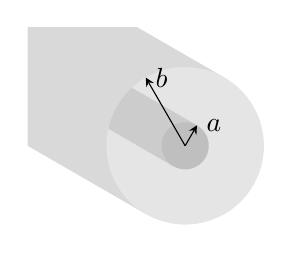
\begin{tikzpicture}
\clip (-2,-1.1) rectangle (1,1.5);
\begin{scope}[rotate=-30]
\fill[gray!30] (-3,-1) rectangle (0,1);
\fill[gray!20] (0,0) circle(1cm);
\begin{scope}
\clip(0,0) circle(1cm);
\fill[gray!40] (-3,-0.3) rectangle (0,0.3);
\fill[gray!50] (0,0) circle(3mm);
\end{scope}
\draw [-stealth] (0, 0) -- (0, 0.3) node[right] {$a$};
\begin{scope}[rotate=60]
\draw [-stealth] (0, 0) -- (0, 1) node[right] {$b$};
\end{scope}
%\draw[-stealth] (120:1) -- node[right,font=\tiny]{$U$}(120:0.2);
%\draw[stealth-] ([yshift=-0.5\pgflinewidth]0,1) -- node[above,font=\tiny]{$I$}([yshift=-0.5\pgflinewidth]0.5,1);
%\draw[-stealth] ([yshift=-0.5\pgflinewidth]0,0) -- node[above,font=\tiny]{$I$}([yshift=-0.5\pgflinewidth]0.5,0);
\end{scope}

\end{tikzpicture}
\end{document}